% !TeX root = main.tex

% ============================================================
% thesis-sync entry: 2026-07-06_bending-characterization-miniaturized
% Type: experimental result
% Insertable section block (no preamble). Requires: graphicx.
% Figure \includegraphics lines are COMMENTED so the file compiles standalone.
% NOTE: quantitative endpoints below are read from the author's plotted data
% (3xSizevsMini.png, centralFiberGraph.png) and from the author's statements;
% intermediate curve values are intentionally not transcribed.
% ============================================================

\section{BENDING CHARACTERIZATION OF THE MINIATURIZED SEGMENT}
\label{sec:lizard-characterization}

\subsection{Experimental Setup}

The pressure--angle characteristic of the isolated three-chambered
segment was measured with the setup previously used for the full-scale
actuator in \cite{TODO-Baschiera-inchworm}: the actuator base is held by
an inverted clamp, a manually operated syringe supplies a single chamber
through an in-line digital pressure sensor with display (PPX series,
CKD), and the deformation is recorded by a video camera. The bending
angle is extracted from the recorded frames by optical measurement. The
actuator bends against gravity in this configuration.

\subsection{Effect of the Threefold Miniaturization}

Figure~\ref{fig:lizard-size-comparison} compares the single-chamber
pressure--angle curves of the full-scale segment (bendable length
$L = 60$~mm) and the miniaturized segment (bendable length $L = 20$~mm);
the bendable length denotes the portion of the
silicone tube not occupied by the end interfaces. Both curves exhibit the
same qualitative shape: a compliant low-pressure region, followed by a
progressively steeper rise of the bending angle beyond approximately
8--10~kPa. The miniaturized segment requires a moderately higher pressure
to reach a given angle over most of the range, reaching approximately
173$^{\circ}$ at 16.4~kPa, whereas the full-scale segment reaches
approximately 182$^{\circ}$ at 14.8~kPa. The threefold reduction in scale
therefore preserves the functional bending range of the actuator at a
comparable, slightly higher, working pressure.

\subsection{Effect of the Central Axial Fiber}

Figure~\ref{fig:lizard-central-fiber} compares the miniaturized segment
with and without the central axial fiber. Below approximately 9~kPa the
two configurations are nearly indistinguishable. Above this pressure the
configuration with the central fiber bends more steeply, reaching
approximately 180$^{\circ}$ at 15.0~kPa, whereas the configuration
without the central fiber reaches approximately 173$^{\circ}$ at
16.4~kPa. The observed behavior is consistent with the intended function
of the fiber: by constraining elongation of the central axis, it converts
a larger share of the chamber inflation into bending curvature in the
high-pressure region, where axial stretch would otherwise grow. The
robot's operating point of approximately 11~kPa lies in the region where
the central-fiber configuration begins to outperform the unconstrained
one. The 180$^{\circ}$ bending capability at 15~kPa refers exclusively to
this isolated single-segment characterization; in the assembled robot the
coupled body--tail unit is operated at approximately 11~kPa, reaching
approximately 75$^{\circ}$ per segment.

% --- Figures (paths to be fixed by the author; commented for compilation) ---
\begin{figure}[tb]
  \centering
  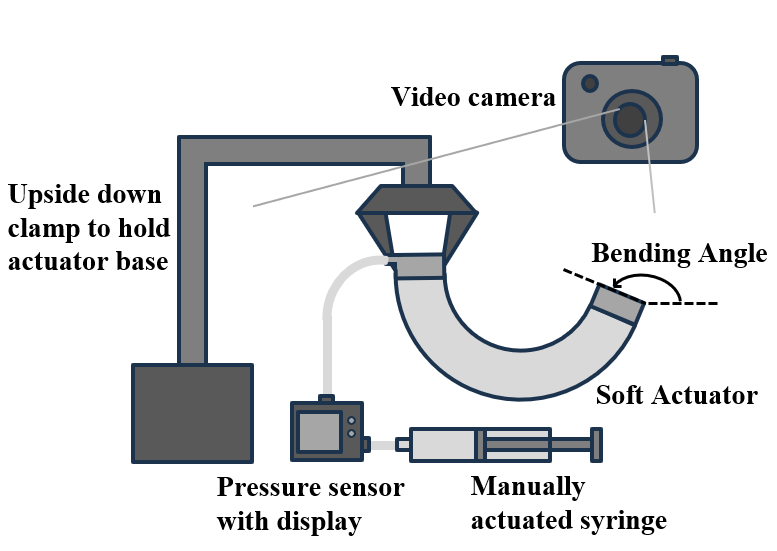
\includegraphics[width=0.9\columnwidth]{figures/experimentalsetup.png}
  \caption{Schematic of the bending characterization setup. The actuator
  base is held by an inverted clamp; a manually actuated syringe supplies
  a single chamber through an in-line pressure sensor with display, and
  the bending angle is extracted optically from the recorded video.}
  \label{fig:lizard-char-setup}
\end{figure}

\begin{figure}[tb]
  \centering
  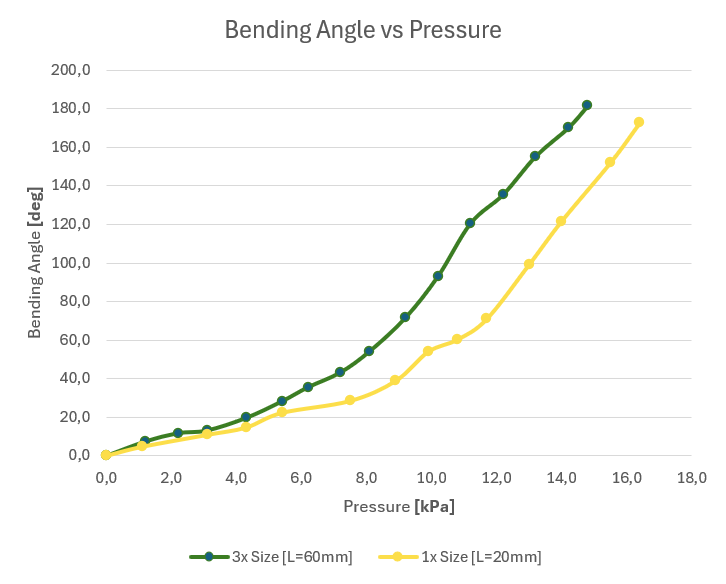
\includegraphics[width=0.9\columnwidth]{figures/3xSizevsMini.png}
  \caption{Single-chamber bending angle versus applied pressure for the
  full-scale segment ($L=60$~mm bendable length) and the miniaturized
  segment ($L=20$~mm bendable length) used in the robot.}
  \label{fig:lizard-size-comparison}
\end{figure}

\begin{figure}[tb]
  \centering
  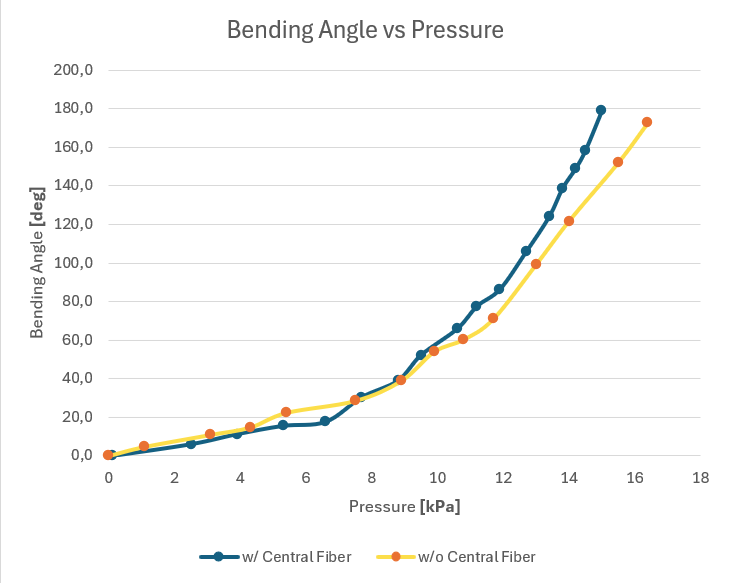
\includegraphics[width=0.9\columnwidth]{figures/centralFiberGraph.png}
  \caption{Single-chamber bending angle versus applied pressure for the
  miniaturized segment with and without the central axial fiber.}
  \label{fig:lizard-central-fiber}
\end{figure}

\begin{figure}[tb]
  \centering
  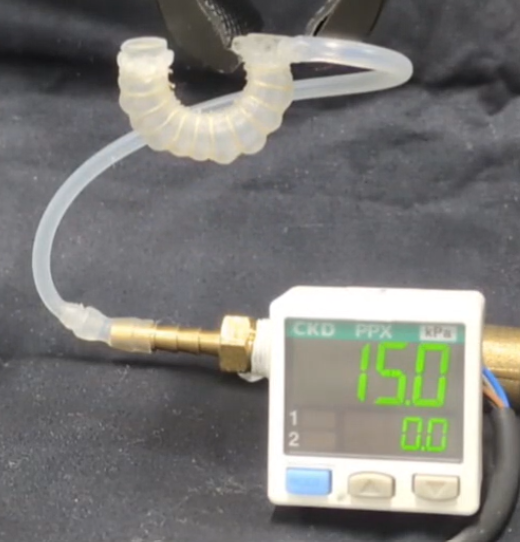
\includegraphics[width=0.75\columnwidth]{figures/centralfiberbendingexperiment.png}
  \caption{The miniaturized segment with central fiber at the
  characterization limit, reaching a bending angle of approximately
  180$^{\circ}$ at an applied pressure of 15.0~kPa.}
  \label{fig:lizard-180deg}
\end{figure}
